% ============================================================================
% REQUIRED PACKAGES & CONFIGURATIONS FOR COMPILING THIS EXPERIMENT:
% ----------------------------------------------------------------------------
% \usepackage{circuitikz}      % For drawing op-amp waveform generator schematics
% \usepackage{pgfplots}        % For generating square and triangular waveforms
% \pgfplotsset{compat=1.18}    % Ensures modern rendering engine defaults
% \usepackage{booktabs}        % For publication-grade tables
% \usepackage{amsmath}         % For mathematical expressions
% \usepackage{siunitx}         % For standard units (\SI, \kilo\omega, \micro\farad)
% ============================================================================

\chapter{Waveform Generation Using Opamps}

\section{Aim}
To design, set up, and study opamp-based waveform generation circuits (Square,  Triangular and Sawtooth Wave Generators) using IC 741. %The specific objectives are:
%\begin{enumerate}
%	\item To implement a non-inverting Schmitt Trigger circuit and measure its upper and lower threshold voltages ($V_{UT}$ and $V_{LT}$).
%	\item To cascade the Schmitt trigger with an inverting integrator to form a closed-loop self-starting relaxation oscillator.
%	\item To experimentally observe, record, and measure the frequency, peak-to-peak amplitude, and phase relationships of the resulting square and triangular output signals.
%	\item To compare theoretical waveform parameters with experimental values.
%\end{enumerate}

\section{Pre-Lab Assignment}
Before conducting the experiment, complete the following analytical problems:
\begin{enumerate}
	%\item Explain how hysteresis in a non-inverting Schmitt trigger prevents noise-induced false triggering at the output.
	%\item For a non-inverting Schmitt trigger powered at $V_{CC} = +15\text{ V}$ and $V_{EE} = -15\text{ V}$ (assuming $V_{sat} = \pm 13.5\text{ V}$), derive the expressions for the upper threshold voltage ($V_{UT}$) and lower threshold voltage ($V_{LT}$) in terms of feedback resistors $R_1$ and $R_2$.
	\item Derive the overall oscillation frequency equation for the square/triangular waveform generator circuits.
%	\begin{equation}
%		f_0 = \frac{R_2}{4 R_1 R C}
%	\end{equation}
	\item Design the waveform generator circuits to produce a $1\text{ kHz}$ square wave and a triangular wave %with a peak-to-peak amplitude of $V_{tri, p-p} = 5.74\text{ V}$, given $C = \SI{0.1}{\micro\farad}$ and $R_1 = \SI{10}{\kilo\Omega}$. Calculate the required values for $R_2$ and $R$.
\end{enumerate}

%\section{Components and Equipment Required}
%The required components and test instruments are listed in Table \ref{tab:components_wavegen}.
%
%\begin{table}[h!]
%	\centering
%	\caption{Components and Equipment Specifications}
%	\label{tab:components_wavegen}
%	\begin{tabular}{llll}
%		\toprule
%		\textbf{S. No.} & \textbf{Item Name} & \textbf{Specification / Range} & \textbf{Quantity} \\
%		\midrule
%		1 & Operational Amplifier & IC 741 (8-pin DIP) & 2 Nos. \\
%		2 & Resistors & \SI{10}{\kilo\Omega}, \SI{12}{\kilo\Omega}, \SI{47}{\kilo\Omega} (1\% Tolerance) & 1 No. each \\
%		3 & Capacitor & \SI{0.1}{\micro\farad} (Metallized Film/Ceramic) & 1 No. \\
%		4 & Dual DC Power Supply & $\pm 15\text{ V}$ fixed/variable & 1 No. \\
%		5 & Digital Storage Oscilloscope & Dual Channel, \SI{20}{\mega\hertz} or higher & 1 No. \\
%		6 & Digital Multimeter & $4\frac{1}{2}$ digit display & 1 No. \\
%		7 & Breadboard \& Wires & Standard setup & As required \\
%		\bottomrule
%	\end{tabular}
%\end{table}

\section{Theory}
\subsubsection{Square wave oscillator}
The basic square wave oscillator is based on the charging and discharging of a capacitor, wired around an op-amp with a positive feedback network. The op-amp's inverting input is the capacitor voltage and the non-inverting input is a portion of the output fed back through resistors $R_1$ and $R_2$ 
(\ref{fig:sqwave_gen}). When the circuit is
first turned on, the capacitor is uncharged, and thus the inverting input is at 0V. This makes the output a positive maximum, and the capacitor begins to charge towards voltage at $V_o$
through resistor $R$. When the capacitor voltage reaches a value equal to the feedback voltage
($V_f$) on the non-inverting input, the op-amp switches to the maximum negative state. At this point, the capacitor begins to discharge from $+V_f$ towards $-V_f$. When the capacitor voltage
reaches $-V_f$, the op-amp switches back to the maximum positive state. This action repeats and a square wave output voltage is obtained.

%A function generator capable of producing synchronized square and triangular waves can be constructed using two op-amps connected in a closed-loop configuration consisting of a **Non-Inverting Schmitt Trigger** (Comparator with positive feedback) and an **Inverting Integrator**.
The Expression for period is:
\[
T=2 RC \ln\dfrac{1+\beta}{1-\beta}
\]

where 
\[
\beta=\dfrac{R_2}{R_1+R_2}
\]

If $R_1 = R_2$, the equation for period reduces to:
\[
T=2 RC \ln 3
\] 
Then, the frequency of oscillation, f:
\[
f=\dfrac{1}{2RC \ln 3}
\] 
\subsubsection{Triangular-wave oscillator}

This circuit (\ref{fig:triangular_wave_ckt}) uses two operational amplifiers. Op-amp A1 functions as a comparator and the op-amp A2 as an integrator. The comparator compares the voltage at point P
continuously with respect to the voltage at the inverting input; which as at ground potential. When the voltage at P goes slightly below zero, the output of A1 will switch to negative
saturation ($-V_{sat}$). Suppose the output of A1 is at positive saturation $+V_{sat}$. Since this voltage is the input of the integrator, the output of A2 will be a negative going ramp. Thus, one end of the voltage divider $R_1-R_2$ is at $+V_{sat}$ and the other at the negative going ramp. At time $t = t_1$, when the negative going ramp attains value of $–V_{ramp}$ the effective voltage at point P becomes slightly less than 0 V. This switches output of A1 from positive saturation to negative saturation level $-V_{sat}$. During the time when the output of A1 is at $-V_{sat}$, the output of A2 increases in the positive direction. At the instant $t = t_2$, the voltage at point P becomes just above
0 V, thereby switching the output of A1 from $-V_{sat}$ to $+V_{sat}$. The cycle repeats and generates a triangular waveform.


At $t=t_1$:
\[
\dfrac{-V_{ramp}}{R_2} = -\dfrac{+V_{sat}}{R_1}
\]
i.e., 
\[
-V_{ramp}=-\dfrac{R_2}{R_1}\left(+V_{sat}\right)
\]

Similarly, at $t-t_2$,
\[
+V_{ramp}=-\dfrac{R_2}{R_1}\left(-V_{sat}\right)
\]
The peak-to-peak output of the triangular wave is:
\[
V_{o(pp)}=+V_{ramp}-\left(-V_{ramp}\right)=2\dfrac{R_2}{R_1}V_{sat}
\]
During the period $0-t_1$, the integrator functions as follows:
\[
V_o(pp) = \dfrac{1}{RC}\int_0^\frac{T}{2}\left(-V_{sat}\right) =\left(\dfrac{V_{sat}}{RC}\right)\left(\dfrac{T}{2}\right)
\]
Then,
\[
T=2RC\dfrac{V_{o(pp)}}{V_{sat}}
\]
Substituting for $V_{o(pp)}$, 
\[]
T=\dfrac{4RCR_2}{R_1}
\]
The frequency of oscillation is then,
\[
f=\dfrac{R_1}{4RCR_2}
\]
%\subsection{Schmitt Trigger Stage (Op-Amp 1)}
%The Schmitt trigger acts as a bi-stable multivibrator with hysteresis. Its non-inverting input receives a combined signal from the output of the integrator ($V_{tri}$) via $R_1$ and its own output ($V_{sq}$) via $R_2$. 
%
%The switching action occurs when the voltage at the non-inverting input terminal crosses $0\text{ V}$ (virtual ground reference). The upper and lower switching threshold levels are given by:
%\begin{equation}
%	V_{UT} = +V_{sat} \left(\frac{R_1}{R_2}\right) \quad \text{and} \quad V_{LT} = -V_{sat} \left(\frac{R_1}{R_2}\right)
%\end{equation}
%The peak-to-peak amplitude of the resulting triangular wave at the output of the second stage is defined by these threshold boundaries:
%\begin{equation}
%	V_{tri, p-p} = V_{UT} - V_{LT} = 2 V_{sat} \left(\frac{R_1}{R_2}\right)
%\end{equation}
\subsubsection{Sawtooth-wave oscillator}
The difference between the triangular and sawtooth waveform is that the rise time of
the triangular wave is always equal to its fall time while in sawtooth wave generator, rise time may be much higher than its fall time or vice versa. The triangular wave generator can be converted to a sawtooth wave generator by injecting a variable dc voltage into the non-inverting terminal of the integrator. This can be done by using a potentiometer as shown in Fig.~\ref{fig:sawtooth_wave_ckt}. When the wiper of the potentiometer is at the centre, the output will be a triangular wave since the duty cycle is 50\%. If the wiper moves towards –V, the rise time of the sawtooth becomes longer than the fall time. If the wiper moves towards +V, the fall time becomes more than the rise time.

%\subsection{Inverting Integrator Stage (Op-Amp 2)}
%The square wave output $V_{sq} = \pm V_{sat}$ from the Schmitt trigger is fed directly into the inverting integrator. Integration of a constant DC voltage yields a linear ramp voltage:
%\begin{equation}
%	V_{tri}(t) = -\frac{1}{RC} \int V_{sq} \, dt
%\end{equation}
%\begin{itemize}
%	\item When $V_{sq} = +V_{sat}$, the integrator output ramps down linearly with a negative slope of $-\frac{V_{sat}}{RC}$.
%	\item When $V_{sq} = -V_{sat}$, the integrator output ramps up linearly with a positive slope of $+\frac{V_{sat}}{RC}$.
%\end{itemize}
%
%\subsection{Frequency Derivation}
%The time required for the triangular wave to ramp from $V_{LT}$ to $V_{UT}$ (half period, $T/2$) is:
%\begin{equation}
%	\frac{T}{2} = \frac{\Delta V_{tri}}{\text{Slope}} = \frac{2 V_{sat} (R_1 / R_2)}{V_{sat} / (RC)} = \frac{2 R_1 R C}{R_2}
%\end{equation}
%Therefore, the total period $T$ and the frequency of oscillation $f_0$ are:
%\begin{equation}
%	T = \frac{4 R_1 R C}{R_2} \implies f_0 = \frac{R_2}{4 R_1 R C}
%\end{equation}

\section{Circuit Diagram}
The complete schematics for the Square, Triangular and Sawtooth Waveform Generators are shown in Figures \ref{fig:sqwave_gen}, \ref{fig:triangular_wave_ckt} and \ref{fig:sawtooth_wave_ckt} respectively.

\begin{figure}
	\centering
	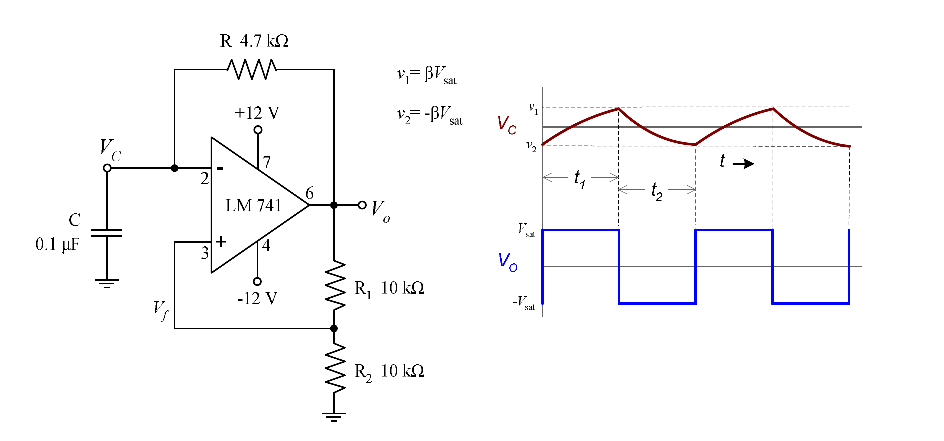
\includegraphics[scale=0.7]{./experiments/figures/opamp_sqwave_gen}
	\caption{Square wave generator and its waveforms}
	\label{fig:sqwave_gen}
\end{figure}

%\begin{figure}[h!]
%	\centering
%	\begin{circuitikz}[scale=0.82, transform shape]
%		% Op-Amp 1: Schmitt Trigger
%		\draw (0,0) node[op amp] (opamp1) {IC 741};
%		\node[font=\tiny, above right] at (opamp1.-) {2};
%		\node[font=\tiny, below right] at (opamp1.+) {3};
%		\node[font=\tiny, above left]  at (opamp1.out) {6};
%		\node[font=\tiny, below right] at (opamp1.up) {7};
%		\node[font=\tiny, above right] at (opamp1.down) {4};
%		
%		% Inverting pin of Op-Amp 1 to Ground
%		\draw (opamp1.-) -- ++(-0.4,0) node[ground] {};
%		
%		% Node S (Summing point for Schmitt trigger inputs)
%		\draw (opamp1.+) -- (-1.8,-0.5) node[circle, fill, inner sep=1.5pt] (nodeS) {};
%		
%		% Op-Amp 1 Output (Square Wave)
%		\draw (opamp1.out) -- (2.2,0) node[circle, fill, inner sep=1.5pt] (vsqNode) {};
%		\draw (vsqNode) -- (2.5,0) node[above] {$V_{sq}$};
%		
%		% Positive Feedback Resistor R2 for Schmitt Trigger
%		\draw (vsqNode) -- (2.2,-1.8) to[R, l_=$R_2\ (\SI{47}{\kilo\Omega})$] (-1.8,-1.8) -- (nodeS);
%		
%		% Path from Vsq to Integrator Input
%		\draw (2.2,0) -- (3.2,0) -- (3.2,0.5) to[R, l=$R\ (\SI{12}{\kilo\Omega})$] (5.2,0.5) -- (5.5,0.5);
%		
%		% Op-Amp 2: Integrator
%		\draw (6.0,0) node[op amp] (opamp2) {IC 741};
%		\node[font=\tiny, above right] at (opamp2.-) {2};
%		\node[font=\tiny, below right] at (opamp2.+) {3};
%		\node[font=\tiny, above left]  at (opamp2.out) {6};
%		\node[font=\tiny, below right] at (opamp2.up) {7};
%		\node[font=\tiny, above right] at (opamp2.down) {4};
%		
%		% Non-inverting pin of Op-Amp 2 to Ground
%		\draw (opamp2.+) -- ++(-0.4,0) node[ground] {};
%		
%		% Feedback Capacitor C for Op-Amp 2
%		\draw (5.2,0.5) node[circle, fill, inner sep=1.5pt] {} -- (5.2,1.8) 
%		to[C, l=$C\ (\SI{0.1}{\micro\farad})$] (7.2,1.8) -- (7.2,0) node[circle, fill, inner sep=1.5pt] {};
%		
%		% Op-Amp 2 Output (Triangular Wave)
%		\draw (opamp2.out) -- (8.0,0) node[circle, fill, inner sep=1.5pt] (vtriNode) {};
%		\draw (vtriNode) -- (8.5,0) node[right] {$V_{tri}$};
%		
%		% Feedback Resistor R1 from Vtri back to Node S
%		\draw (8.0,0) -- (8.0,-3.2) to[R, l_=$R_1\ (\SI{10}{\kilo\Omega})$] (-1.8,-3.2) -- (nodeS);
%		
%		% Vertical Power Lines for Op-Amp 1
%		\draw (opamp1.up) -- ++(0,0.4) node[above, font=\tiny] {$+15\text{V}$};
%		\draw (opamp1.down) -- ++(0,-0.4) node[below, font=\tiny] {$-15\text{V}$};
%		
%		% Vertical Power Lines for Op-Amp 2
%		\draw (opamp2.up) -- ++(0,0.4) node[above, font=\tiny] {$+15\text{V}$};
%		\draw (opamp2.down) -- ++(0,-0.4) node[below, font=\tiny] {$-15\text{V}$};
%	\end{circuitikz}
%	\caption{Op-Amp Based Square and Triangular Wave Generator Schematic}
%	\label{fig:wavegen_circuit}
%\end{figure}

\begin{figure}
	\centering
	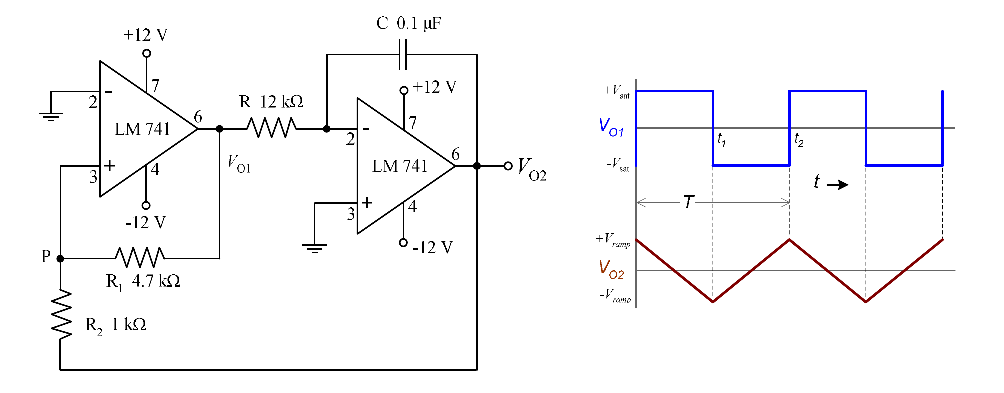
\includegraphics[scale=0.7]{./experiments/figures/opamp_triangular_wave_gen}
	\caption{Triangular wave generator circuit and waveforms}
	\label{fig:triangular_wave_ckt}
\end{figure}

\begin{figure}
	\centering
	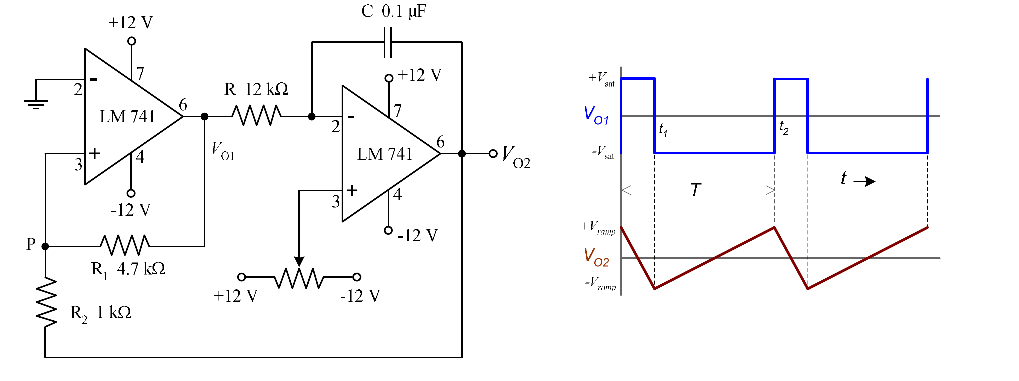
\includegraphics[scale=0.7]{./experiments/figures/opamp_sawtooth_wave_gen}
	\caption{Sawtooth wave generator circuit and waveforms}
	\label{fig:sawtooth_wave_ckt}
\end{figure}

\section{Design}
\begin{itemize}
	\item Target Frequency: $f_0 = 1\text{ kHz}$
	\item Power Supply: $V_{CC} = +12\text{ V}$, $V_{EE} = -12\text{ V} \implies V_{sat} \approx \pm 10\text{ V}$
	\item Desired Peak-to-Peak Triangular/Sawtooth Amplitude: $V_{tri, p-p} = 5\text{ V}$
\end{itemize}
\subsection{Design of square wave generator}
Take $\beta=0.5$ and $R_1=R_2=\SI{10}{\kilo\Omega}$.
	Frequency,
	\[
	f=\dfrac{1}{RC\ln 3}
	\]
	Assume $C=\SI{0.1}{\micro F}$.
	Then,
	\[
	R = \dfrac{1}{2Cf\ln 3} = \dfrac{1}{2\times 0.1\times 10^{-6}\times1000\times\ln 3} = \SI{4.55}{\kilo\ohm}
	\]
	Select standard value of $\SI{4.7}{\kilo\ohm}$ for $R$.
\subsection{Design of triangular wave generator}
The frequency,
\[
f=\dfrac{R_1}{4RCR_2}
\] and
\[
V_{o(pp)}=2\dfrac{R_2}{R_1}V_{sat}
\]
As before, $V_{sat}\approx 10 \text{V}$. Assume $R_2=\SI{1}{\kilo\ohm}$. 
%

Then,
\[
R_1=2\dfrac{V_{sat}}{V_{o(pp)}} R_2 = \dfrac{2\times 10}{5}\times 1\times 10^3 = \SI{4}{\kilo\ohm}
\]

Select standard value, $R_1=\SI{4.7}{\kilo\ohm}$.

Assume $C=\SI{0.1}{\micro F}$.
\[
R=\dfrac{R_1}{4fCR_2} = \dfrac{4.7\times10^3}{4\times1000\times0.1\times10^{-6}\times1\times10^3} = \SI{11.7}{\kilo\ohm}
\]
Select standard value, $R=\SI{12}{\kilo\ohm}$.
\subsubsection{Design of sawtooth wave generator}
Design is similar to that of triangle wave generator. Select $R_3=\SI{47}{\kilo\ohm}$ potentiometer to vary the reference voltage of second op-amp.
%%\subsection{Calculations}
%\begin{enumerate}
%	\item Select $R_1 = \SI{10}{\kilo\Omega}$. Calculate $R_2$ for the desired triangular output swing:
%	\begin{equation}
%		V_{tri, p-p} = 2 V_{sat} \left(\frac{R_2}{R_1}\right) \implies 5.74\text{ V} = 2(13.5\text{ V}) \left(\frac{\SI{10}{\kilo\Omega}}{R_2}\right)
%	\end{equation}
%	\begin{equation}
%		R_2 = \frac{27 \times 10^4}{5.74} \approx \SI{47}{\kilo\Omega} \quad (\text{Standard 1\% Resistor})
%	\end{equation}
%	
%	\item Calculate threshold voltages:
%	\begin{equation}
%		V_{UT} = +13.5 \times \left(\frac{10}{47}\right) = +2.87\text{ V}, \quad V_{LT} = -13.5 \times \left(\frac{10}{47}\right) = -2.87\text{ V}
%	\end{equation}
%	
%	\item Select $C = \SI{0.1}{\micro\farad}$. Calculate $R$ for $f_0 = 1\text{ kHz}$:
%	\begin{equation}
%		f_0 = \frac{R_2}{4 R_1 R C} \implies R = \frac{R_2}{4 R_1 f_0 C} = \frac{47 \times 10^3}{4 \times (10 \times 10^3) \times 1000 \times (0.1 \times 10^{-6})} = \SI{11.75}{\kilo\Omega}
%	\end{equation}
%	Select standard resistor value $R = \SI{12}{\kilo\Omega}$.
%	
%	\item Recalculate theoretical frequency with selected standard components:
%	\begin{equation}
%		f_{0,\text{theoretical}} = \frac{47 \times 10^3}{4 \times (10 \times 10^3) \times (12 \times 10^3) \times (0.1 \times 10^{-6})} = \SI{979.17}{\text{Hz}}
%	\end{equation}
%\end{enumerate}

\section{Procedure}
\begin{enumerate}
	\item Set up the circuit after testing the components.
	\item Set up the square wave generator as shown in figure and observe the output waveform and note down their amplitudes and frequency.
	\item Set up the triangular wave generator as shown in figure and observe the output waveform parameters.
	\item Set up the sawtooth wave generator as shown in figure and note down the frequency, amplitude, rise time and fall time.
	\item Move the wiper of the potentiometer in both directions and observe the changes
	taking place in the waveform.
\end{enumerate}


%\begin{enumerate}
%
%\item Wire the waveform generator circuit on the breadboard as per the schematic in Figure \ref{fig:wavegen_circuit}.
%\item Connect $\pm 15\text{ V}$ regulated DC power supply connections to pins 7 and 4 of both IC 741 packages.
%\item Connect Channel 1 of the DSO to the Schmitt Trigger output ($V_{sq}$, Pin 6 of IC 741 \#1) and Channel 2 to the Integrator output ($V_{tri}$, Pin 6 of IC 741 \#2).
%\item Set DSO channels to DC coupling and adjust vertical scale to capture both waveforms simultaneously.
%\item Measure the peak-to-peak amplitudes ($V_{sq, p-p}$ and $V_{tri, p-p}$) and the period $T$ of the output waveforms.
%\item Calculate the experimental frequency $f_0 = 1/T$ and compare it with $f_{0,\text{theoretical}}$.
%\item Verify the switching points on the DSO in X-Y mode to plot the hysteresis loop ($V_{sq}$ vs. $V_{tri}$) and measure $V_{UT}$ and $V_{LT}$.
%\end{enumerate}

%\section{Precautions}
%\begin{enumerate}
%	\item Ensure dual power supply polarity ($\pm 15\text{ V}$) is double-checked before powering the circuit to prevent destroying the ICs.
%\item Connect Schmitt trigger positive feedback to non-inverting pin 3 and integrator negative feedback to inverting pin 2.
%\item Verify that the op-amps do not overheat during continuous operation.
%\end{enumerate}

%\section{Model Graph / Expected Waveforms}
%Figure \ref{fig:expected_waveforms} shows the expected time-aligned square and triangular output waveforms.
%
%\begin{figure}[h!]
%\centering
%\begin{tikzpicture}
%\begin{axis}[
%	axis lines=middle,
%	xlabel={$t\text{ (ms)}$},
%	ylabel={Voltage (V)},
%	xmin=0, xmax=2.0,
%	ymin=-16, ymax=16,
%	grid=both,
%	grid style={line width=.1pt, draw=gray!20},
%	major grid style={line width=.2pt, draw=gray!40},
%	width=11.5cm, height=6.5cm,
%	title={\textbf{Expected Time-Synchronized Square and Triangular Waveforms}},
%	legend pos=outer north east,
%	legend style={font=\footnotesize}
%	]
%	% Square Wave Output Vsq (+-13.5V, T = 1.02 ms)
%	\addplot[ultra thick, blue] coordinates {
%		(0, 13.5) (0.51, 13.5) (0.51, -13.5) (1.02, -13.5) 
%		(1.02, 13.5) (1.53, 13.5) (1.53, -13.5) (2.04, -13.5)
%	};
%	\addlegendentry{$V_{sq}\ (\pm 13.5\text{ V})$}
%	
%	% Triangular Wave Output Vtri (+-2.87V)
%	\addplot[ultra thick, red, dashed] coordinates {
%		(0, -2.87) (0.51, 2.87) (1.02, -2.87) (1.53, 2.87) (2.04, -2.87)
%	};
%	\addlegendentry{$V_{tri}\ (\pm 2.87\text{ V})$}
%\end{axis}
%\end{tikzpicture}
%\caption{Synchronized Output Waveforms of the Generator Circuit}
%\label{fig:expected_waveforms}
%\end{figure}
%
%\section{Observation Tables}
%
%\subsection{Waveform Parameters}
%Record the measured amplitude and frequency parameters in Table \ref{tab:obs_waveforms}.
%
%\begin{table}[h!]
%\centering
%\caption{Theoretical vs Practical Waveform Measurements}
%\label{tab:obs_waveforms}
%\begin{tabular}{lcccc}
%\toprule
%\textbf{Parameter} & \textbf{Theoretical Value} & \textbf{Measured Value} & \textbf{\% Error} \\
%\midrule
%Square Wave Peak-to-Peak ($V_{sq, p-p}$) & $27.0\text{ V}$ & & \\
%Triangular Wave Peak-to-Peak ($V_{tri, p-p}$) & $5.74\text{ V}$ & & \\
%Time Period ($T$) & $1.02\text{ ms}$ & & \\
%Frequency ($f_0$) & \SI{979.17}{\text{Hz}} & & \\
%\bottomrule
%\end{tabular}
%\end{table}
%
%\subsection{Hysteresis Threshold Voltages}
%Record threshold voltage observations in Table \ref{tab:obs_thresholds}.
%
%\begin{table}[h!]
%\centering
%\caption{Schmitt Trigger Threshold Verification}
%\label{tab:obs_thresholds}
%\begin{tabular}{lccc}
%\toprule
%\textbf{Threshold Level} & \textbf{Theoretical Voltage} & \textbf{Measured Voltage} & \textbf{\% Error} \\
%\midrule
%Upper Threshold ($V_{UT}$) & $+2.87\text{ V}$ & & \\
%Lower Threshold ($V_{LT}$) & $-2.87\text{ V}$ & & \\
%Hysteresis Width ($V_H = V_{UT} - V_{LT}$) & $5.74\text{ V}$ & & \\
%\bottomrule
%\end{tabular}
%\end{table}

\section{Result}
The circuits of op-amp square, triangular and sawtooth waveform generators were successfully designed, constructed, and tested.
%\begin{itemize}
%\item The experimental oscillation frequency was measured as $f_{0,\text{practical}} = \rule{2cm}{0.15mm}\text{ Hz}$, showing a percentage error of \rule{1.5cm}{0.15mm}\% compared to the theoretical frequency of \SI{979.17}{\text{Hz}}.
%\item The triangular wave peak-to-peak amplitude was measured as $V_{tri, p-p} = \rule{2cm}{0.15mm}\text{ V}$ with threshold limits $V_{UT} = \rule{1.5cm}{0.15mm}\text{ V}$ and $V_{LT} = \rule{1.5cm}{0.15mm}\text{ V}$.
%\end{itemize}

\section{Questions}
\begin{enumerate}
	\item How does varying resistor $R$ affect the frequency and amplitude of the triangular wave?
\item What limits the maximum achievable operating frequency of this waveform generator circuit?
%\item How can the circuit be modified to produce a variable duty cycle (asymmetric triangle / sawtooth wave)?
\item Why is a non-inverting Schmitt trigger preferred over an inverting Schmitt trigger in the specific two-stage triangle/sawtooth generator topology?
\item How does op-amp slew rate ($\text{SR} = \SI{0.5}{\volt/\micro\second}$ for IC 741) distort the square wave output at high frequencies?
\end{enumerate}